\documentclass[]{article}
\usepackage{lmodern}
\usepackage{amssymb,amsmath}
\usepackage{ifxetex,ifluatex}
\usepackage{fixltx2e} % provides \textsubscript
\ifnum 0\ifxetex 1\fi\ifluatex 1\fi=0 % if pdftex
  \usepackage[T1]{fontenc}
  \usepackage[utf8]{inputenc}
\else % if luatex or xelatex
  \ifxetex
    \usepackage{mathspec}
  \else
    \usepackage{fontspec}
  \fi
  \defaultfontfeatures{Ligatures=TeX,Scale=MatchLowercase}
\fi
% use upquote if available, for straight quotes in verbatim environments
\IfFileExists{upquote.sty}{\usepackage{upquote}}{}
% use microtype if available
\IfFileExists{microtype.sty}{%
\usepackage{microtype}
\UseMicrotypeSet[protrusion]{basicmath} % disable protrusion for tt fonts
}{}
\usepackage[margin=1in]{geometry}
\usepackage{hyperref}
\hypersetup{unicode=true,
            pdftitle={Molecular and greenhouse validation of field evolved resistance to glyphosate and PPO-inhibitors in Palmer amaranth populations},
            pdfauthor={Maxwel C Oliveira and Rodrigo Werle},
            pdfborder={0 0 0},
            breaklinks=true}
\urlstyle{same}  % don't use monospace font for urls
\usepackage{longtable,booktabs}
\usepackage{graphicx,grffile}
\makeatletter
\def\maxwidth{\ifdim\Gin@nat@width>\linewidth\linewidth\else\Gin@nat@width\fi}
\def\maxheight{\ifdim\Gin@nat@height>\textheight\textheight\else\Gin@nat@height\fi}
\makeatother
% Scale images if necessary, so that they will not overflow the page
% margins by default, and it is still possible to overwrite the defaults
% using explicit options in \includegraphics[width, height, ...]{}
\setkeys{Gin}{width=\maxwidth,height=\maxheight,keepaspectratio}
\IfFileExists{parskip.sty}{%
\usepackage{parskip}
}{% else
\setlength{\parindent}{0pt}
\setlength{\parskip}{6pt plus 2pt minus 1pt}
}
\setlength{\emergencystretch}{3em}  % prevent overfull lines
\providecommand{\tightlist}{%
  \setlength{\itemsep}{0pt}\setlength{\parskip}{0pt}}
\setcounter{secnumdepth}{5}
% Redefines (sub)paragraphs to behave more like sections
\ifx\paragraph\undefined\else
\let\oldparagraph\paragraph
\renewcommand{\paragraph}[1]{\oldparagraph{#1}\mbox{}}
\fi
\ifx\subparagraph\undefined\else
\let\oldsubparagraph\subparagraph
\renewcommand{\subparagraph}[1]{\oldsubparagraph{#1}\mbox{}}
\fi

%%% Use protect on footnotes to avoid problems with footnotes in titles
\let\rmarkdownfootnote\footnote%
\def\footnote{\protect\rmarkdownfootnote}

%%% Change title format to be more compact
\usepackage{titling}

% Create subtitle command for use in maketitle
\newcommand{\subtitle}[1]{
  \posttitle{
    \begin{center}\large#1\end{center}
    }
}

\setlength{\droptitle}{-2em}

  \title{Molecular and greenhouse validation of field evolved resistance to
glyphosate and PPO-inhibitors in Palmer amaranth populations}
    \pretitle{\vspace{\droptitle}\centering\huge}
  \posttitle{\par}
    \author{Maxwel C Oliveira and Rodrigo Werle}
    \preauthor{\centering\large\emph}
  \postauthor{\par}
      \predate{\centering\large\emph}
  \postdate{\par}
    \date{10/29/2018}


\begin{document}
\maketitle

\tableofcontents 

\pagebreak

\section{Molecular work}\label{molecular-work}

Leaf tissue samples from 51 Palmer amaranth populations (5 plants
population\textsuperscript{-1}) were collected at multiple counties in
SW Nebraska in the fall of 2017. The samples were stored at -80C until
used for a molecular screening at the University of Illinois-Urbana
Champaign. Genomic DNA was extracted from five samples per population
and samples were tested for the presence of the PPO glycine 210 deletion
(G210), which is known to confer resistance to PPO herbicides in Palmer
amaranth. Samples were also tested for genomic copy numbers of the EPSPS
gene (an increase in genomic copy number of EPSPS is known to confer
glyphosate resistance in Palmer amaranth). According to the molecular
results of 51 Palmer amaranth populations, 59\% of the populations had
at least one sample positive for resistance to PPO-inhibiting
herbicides. Forty-seven percent of Palmer amaranth populations tested
positive for resistance to glyphosate. Moreover, 27\% of the populations
tested positive for resistance to both herbicide groups (Figure 1 and
Table 1).

\begin{figure}[h]

{\centering 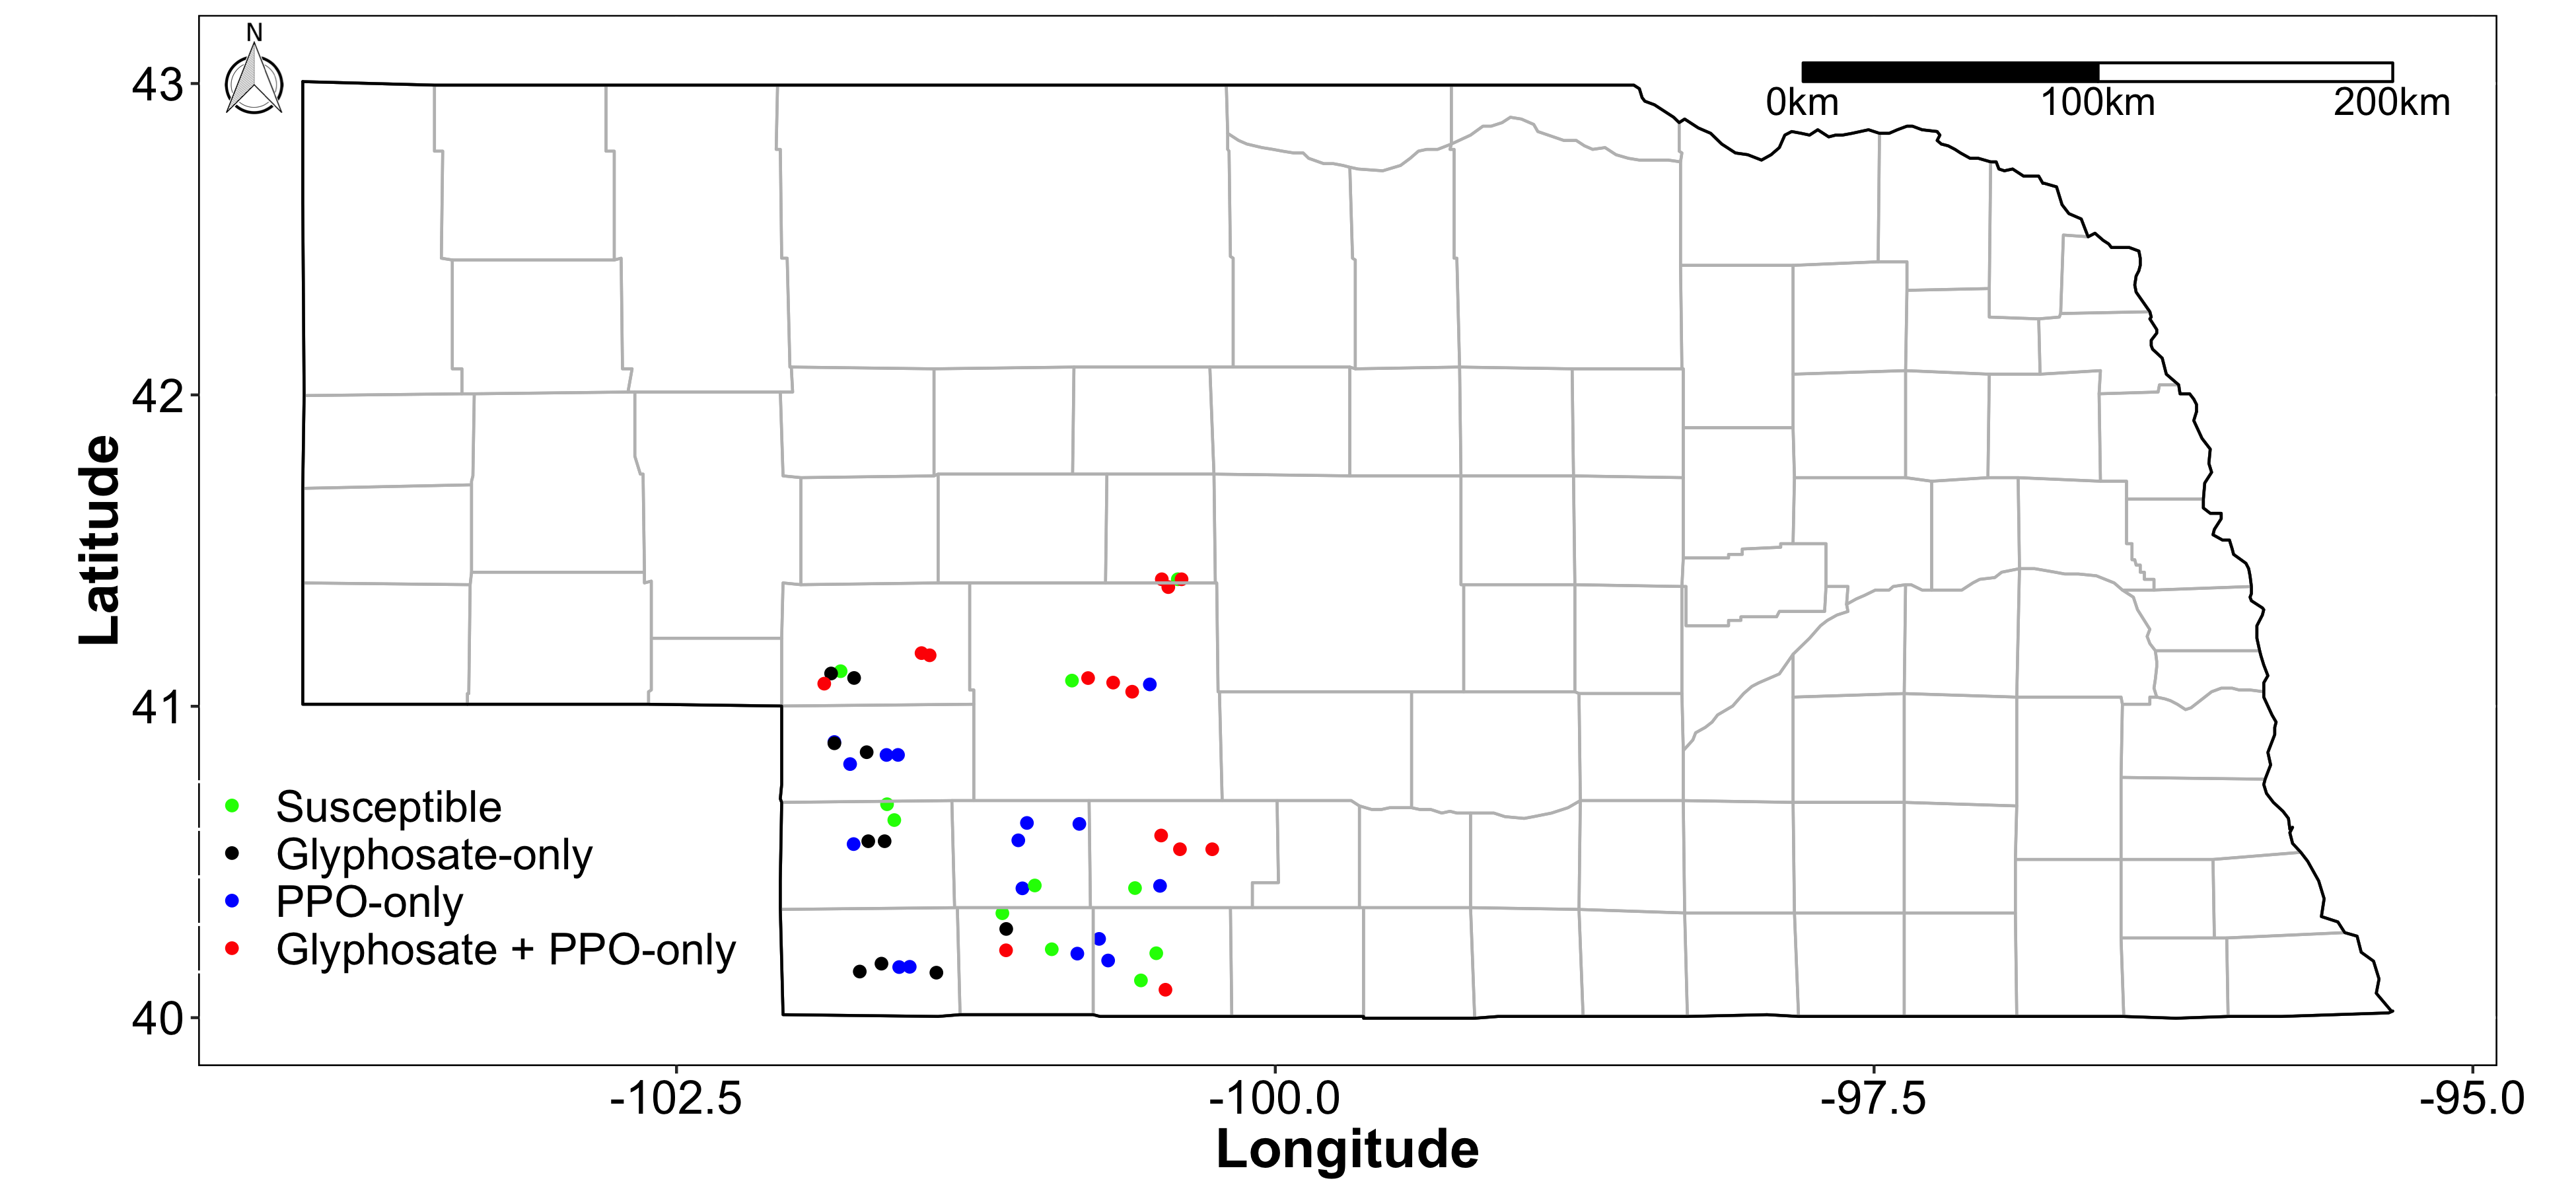
\includegraphics[width=0.9\linewidth]{map} 

}

\caption{Distribution of EPSPS- and PPO-inhibiting herbicide resistance in Palmer amaranth populations from SW Nebraska according to molecular assays.}\label{fig:unnamed-chunk-1}
\end{figure}

Herein, the percentage of Palmer amaranth populations with PPO and/or
EPSPS resistance was reported as:

Equation 1: \[Y=\frac{R}{T} * 100 \]

where \emph{Y} is the \% of PPO or EPSPS resistant Palmer amararanth
population in the molecular study; \emph{R} is the number of plants with
a PPO mutation or showing more than 2 EPSPS copy number; and \emph{T} is
the total number of samples for each population used in the molecular
study (5 plants).

\pagebreak

\begin{longtable}[]{@{}lll@{}}
\caption{Results of the molecular screening for PPO and EPSPS resistance
in Palmer amaranth populations from Nebraska.}\tabularnewline
\toprule
Population\textsuperscript{1} & PPO mutation & EPSPS gene copy
\#\tabularnewline
\midrule
\endfirsthead
\toprule
Population\textsuperscript{1} & PPO mutation & EPSPS gene copy
\#\tabularnewline
\midrule
\endhead
CHA1 & None & 1\tabularnewline
CHA2 & None & 1\tabularnewline
\textbf{CHA3} & None & 12\tabularnewline
CHA4 & R128G het & 23\tabularnewline
CHA5 & PPX2\_G210 & 1\tabularnewline
DUN1 & PPX2\_G210 & 8\tabularnewline
DUN2 & PPX2\_G210 & 1\tabularnewline
\textbf{DUN3} & PPX2\_G210 & 1\tabularnewline
\textbf{DUN4} & None & 6\tabularnewline
\textbf{DUN5} & PPX2\_G210 & 24\tabularnewline
FRO1 & PPX2\_G210 & 6\tabularnewline
FRO2 & PPX2\_G210 & 6\tabularnewline
FRO3 & PPX2\_G210 & 11\tabularnewline
FRO4 & PPX2\_G210 & 1\tabularnewline
FRO5 & None & 1\tabularnewline
\textbf{HAY1} & PPX2\_G210 & 1\tabularnewline
HAY2 & PPX2\_G210 & 3\tabularnewline
\textbf{HAY3} & PPX2\_G210 & 1\tabularnewline
\textbf{HAY4} & PPX2\_G210 & 1\tabularnewline
HAY5 & None & 1\tabularnewline
HIT1 & None & 20\tabularnewline
HIT2 & None & 30\tabularnewline
HIT3 & PPX2\_G210 & 6\tabularnewline
HIT4 & None & 3\tabularnewline
HIT5 & PPX2\_G210 & 1\tabularnewline
KEI1 & PPX2\_G210 & 38\tabularnewline
\textbf{KEI2} & PPX2\_G210 & 12\tabularnewline
\textbf{KEI3} & None & 1\tabularnewline
KEI4 & None & 14\tabularnewline
\textbf{KEI5} & PPX2\_G210 & 7\tabularnewline
\textbf{KEI6} & None & 21\tabularnewline
LIN1 & PPX2\_G210 & 1\tabularnewline
LIN2 & PPX2\_G210 & 5\tabularnewline
LIN3 & PPX2\_G210 & 5\tabularnewline
LIN4 & PPX2\_G210 & 4\tabularnewline
LIN5 & None & 1\tabularnewline
\textbf{LOG1} & PPX2\_G210 & 50\tabularnewline
\textbf{LOG2} & None & 1\tabularnewline
LOG3 & PPX2\_G210 & 6\tabularnewline
\textbf{LOG4} & PPX2\_G210 & 5\tabularnewline
PER1 & PPX2\_G210 & 1\tabularnewline
\textbf{PER2} & None & 39\tabularnewline
PER3 & None & 1\tabularnewline
\textbf{PER4} & None & 14\tabularnewline
PER5 & PPX2\_G210 & 1\tabularnewline
PER6 & PPX2\_G210 & 1\tabularnewline
RED1 & PPX2\_G210 & 1\tabularnewline
\textbf{RED2} & PPX2\_G210 & 3\tabularnewline
RED3 & R128G het & 6\tabularnewline
\textbf{RED4} & PPX2\_G210 & 5\tabularnewline
\textbf{RED5} & None & 1\tabularnewline
\bottomrule
\end{longtable}

\textsuperscript{1} Populations in bold were also screened for
resistance in the greenhouse.

\pagebreak

\section{Greenhouse validation}\label{greenhouse-validation}

The objective of this study was to validade the molecular results of PPO
and EPSPS resistance in Palmer amaranth populations with PPO-(fomesafen
and lactofen) and EPSPS-(glyphosate) inhibiting herbicide treatments.
Nineteen out 51 Palmer amaranth populations were sected for the
greenhouse study (Table 1). Palmer amaranth were germinated in trays
containing potting mix and seedlings were tansplanted to cone-tainers at
0.5 cm tall (1--2 leaf stage). The experimental unit was a single
cone-tainer with a Palmer amaranth seedling. When plants reached 8-10 cm
tall, the herbicide treatment was perfomerd at 1x the recommended rate
(Table 2). Each experimental run consisted of 20 plants of each Palmer
amaranth population per herbicide. We conducted exprimental runs in the
winter, summer, and fall (Table 3).

\begin{longtable}[]{@{}lll@{}}
\caption{Herbicide and rate used in the greenhouse study at the
University of Wisconsin-Madison.}\tabularnewline
\toprule
Herbicide & Trade Name & Rate (g ae(ai)
ha\textsuperscript{-1})\tabularnewline
\midrule
\endfirsthead
\toprule
Herbicide & Trade Name & Rate (g ae(ai)
ha\textsuperscript{-1})\tabularnewline
\midrule
\endhead
Glyphosate & Roundup WeatherMax & 870\tabularnewline
Fomesafen & Flexstar & 225.6\tabularnewline
Lactofen & Cobra & 218.8\tabularnewline
\bottomrule
\end{longtable}

Twenty-one days after herbicide treatment, Palmer amaranth plants were
rated based on a scale from 1 to 10 as descrebed in Figure 2 (PPO
inhibiting herbicides) and Figure 3 (EPSPS-inhibiting herbicides). A
plant rated 1 to 3, 4 to 7, or 8 to 10, was considered susceptible,
medium, or with low injury, respectively. Palmer amaranth seedlings
classified with medium and low injury were reported as resistant to
herbicide field rate (``practical resistance''); therefore, the
percentage of resistant seedlings of each population was calculated:

Equation 2: \[Z=\frac{R}{T} * 100 \]

where \emph{Z} is the \% of PPO or EPSPS resistance in plants within
Palmer amaranth population in the greenhouse; \emph{R} is the sum of
Palmer amaranth seedlings showing medium (4 to 7) to low (8 to 10)
injury; and \emph{T} is the total number of Palmer amaranth plants
treated with herbicide for each population (20 plants).

\begin{longtable}[]{@{}lll@{}}
\caption{Experimental runs of the greenhouse screening with glyphosate,
fomesafen, and lactofen at the University of
Wisconsin-Madison.}\tabularnewline
\toprule
Run & Months & Herbicide\tabularnewline
\midrule
\endfirsthead
\toprule
Run & Months & Herbicide\tabularnewline
\midrule
\endhead
Spring & March to April & glyphosate and fomesafen\tabularnewline
Summer & June to July & glyphosate and fomesafen\tabularnewline
Fall & August to September & fomesafen and lactofen\tabularnewline
\bottomrule
\end{longtable}

\begin{figure}[h]

{\centering \includegraphics[width=0.8\linewidth]{PPO} 

}

\caption{PPO-inhibiting herbicides (Fomesafen and Lactofen) injury rate evaluation at 21 days after treatment.}\label{fig:unnamed-chunk-2}
\end{figure}

\begin{figure}[h]

{\centering 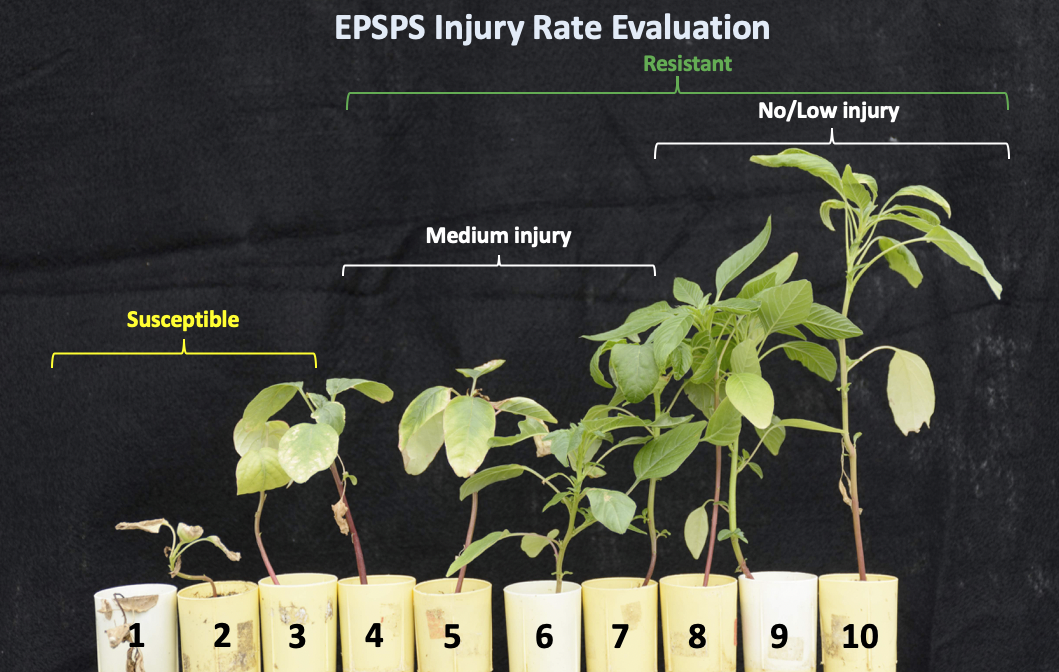
\includegraphics[width=0.8\linewidth]{EPSPS} 

}

\caption{EPSPS-inhibiting herbicides (glyphosate) injury rate evaluation at 21 days after treatment.}\label{fig:unnamed-chunk-3}
\end{figure}

\section{Statistical analysis}\label{statistical-analysis}

The \emph{Y} and \emph{Z} results for the 19 Palmer amaranth populations
were regressed (\emph{geom\_smooth}) using \emph{ggplot2} package in R
statistical software. Also, the Pearson-correlation was performed to
test the hypothesis that results from the molecular work match the
greenhouse assay.

\section{Results}\label{results}

\subsection{Glyphosate-resistance}\label{glyphosate-resistance}

Results showed correlation of 0.43 and 0.86 in the winter and summer,
respectively (figure 4). Conducting the greenhouse assay during winter
time might be masking the correlation results. When plants were screened
during the summer, a stong correlation (P=0.00) between the results from
the greenhouse and moelcular assays was detected.

\begin{figure}
\centering
\includegraphics{Report_files/figure-latex/unnamed-chunk-4-1.pdf}
\caption{Regression between the glyphosate molecular and greenhouse
assays. Result is presented for run in winter (left) and summer (right)
timings.}
\end{figure}

\subsection{PPO-resistance}\label{ppo-resistance}

\subsubsection{Fomesafen screening}\label{fomesafen-screening}

Results from the PPO screening with fomesafen in Palmer amaranth showed
no to low correlation between the greenhouse and molecular assays
(Figure 5). The highest correlation (0.40; P=0.09) was in the
experimental run conducted in the fall.

\begin{figure}
\centering
\includegraphics{Report_files/figure-latex/unnamed-chunk-6-1.pdf}
\caption{Regression between the result from the fomesafen molecular and
greenhouse assays. Result is presented for run in winter (left), summer
(center), and fall (right) timings.}
\end{figure}

\subsubsection{Lactofen screening}\label{lactofen-screening}

There was no to low correlation between molecular and greenhouse assays
with fomesafen (Figure 4). This result led us to raise the hypothesis
thatfomesafen was not a good indicator to compare to the molecular
results for PPO resistance. Therefore, we conducted an experimental run
using lactofen, a more effective herbice (acording to field evaluation)
in the diphenyl-ether family. However, for lactofen, results showed
-0.38 (P=0.10) correlation between greenhouse and molecular assays with
(Figure 6).

\begin{figure}
\centering
\includegraphics{Report_files/figure-latex/unnamed-chunk-8-1.pdf}
\caption{Regression between the lactofen molecular and greenhouse
studies. Result is presented for run in winter (left), summer (center),
and fall (right) timings.}
\end{figure}

\subsubsection{Fomesafen and Lactofen
correlation}\label{fomesafen-and-lactofen-correlation}

There was no significant correlation between fomesafen and lactofen
(0.36; P=0.14) (Figure 7).

\begin{figure}
\centering
\includegraphics{Report_files/figure-latex/unnamed-chunk-10-1.pdf}
\caption{Regression between the fomesafen and lacotfen greenhouse
assays. Result is presented for a run in fall timing.}
\end{figure}

\section{Take-home message}\label{take-home-message}

\begin{itemize}
\item
  Results from greenhouse assays varied across experimental runs.
\item
  High correlation detected between molecular (EPSPS copy number) and
  greenhouse assays for the Palmer amaranth populations tested herein.
\item
  Thus, the molecular assay is an excellent technique for rapid
  detection of glyphosate resistance in Palmer amaranth.
\item
  Lack of correlation between molecular and greenhouse assays was
  detected herein; this indicates that not all plants positive for PPO
  resistance in molecular assays will necessarily be resistant to a
  label rate application in the field.
\item
  Perhaps the tested Palmer amaranth populations are segregating for PPO
  resistance which may, in parts, explain the lack of correlation found
  herein. Thoughts?
\end{itemize}

\pagebreak

\section{\texorpdfstring{\textbf{Abstract
NCWSS}}{Abstract NCWSS}}\label{abstract-ncwss}

Maxwel Coura Oliveira\textsuperscript{1}, Darci
Giacomini\textsuperscript{2}, Nikola Arsenijevic\textsuperscript{2},
Gustavo Vieira\textsuperscript{3}, Patrick Tranel\textsuperscript{2},
Rodrigo Werle\textsuperscript{1}

\textsuperscript{1}University of Wisconsin-Madison,
\textsuperscript{2}University of Illinois-Urbana Champaign,
\textsuperscript{3}University of Nebraska-Lincoln

\textbf{Abstract}: Palmer amaranth (\emph{Amaranthus palmeri}) is the
most troublesome weed species in row crop production areas across the
United States. It has extended emergence window and vigorous growth,
which make control with POST-emergence herbicides difficult. Growers
have reported that POST herbicide applications in RR soybean systems,
which include glyphosate and/or PPO inhibitors, are not providing
adequate levels of Palmer amaranth control. Unsatisfactory levels of
Palmer amaranth control may not be exclusively due to herbicide
resistance. In some cases, poor Palmer amaranth control is a result of
improper herbicide application, weed size, and/or adverse environmental
conditions. Therefore, the objective of this study was to validate,
under greenhouse conditions, the results of molecular confirmation of
PPO and EPSPS resistance in Palmer amaranth populations. Nineteen Palmer
amaranth populations from western Nebraska were used in this study with
20 seedlings herbicide\textsuperscript{-1} run\textsuperscript{-1},
which was conducted during winter, summer, and fall. Palmer amaranth
seedlings were treated at 8-10 cm tall with EPSPS-(glyphosate) and PPO-
(fomesafen and lactofen) inhibiting herbicides at the field recommended
rate. At 21 days after herbicide treatment, plants were evaluated as
dead (susceptible) or alive (resistant). Pearson-correlation was
performed to evaluate if greenhouse screenings match the results from
the molecular assay. Results showed strong correlation between
greenhouse and molecular assays (EPSPS gene copy number) for glyphosate
resistance. The correlation was higher (0.86; P\textless{}0.01) when
Palmer amaranth plants were screened in summer versus winter (0.43;
p=0.06). Greenhouse screening for fomesafen (PPO resistance) did not
correlate to results from molecular assays (\_G210 deletion). The
highest correlation for fomesafen (PPO resistance) was in the fall run
(0.40; P=0.09). Lactofen was used to investigate whether the PPO results
deviate by herbicide within the PPO-inhibiting herbicides. Lactofen
demonstrated similar results to fomesafen but negative correlation
(-0.38; P=0.10) with the molecular study. Therefore, the use of
molecular techniques for detection of glyphosate resistance in Palmer
amaranth is robust and accurate, but not necessarily for PPO-inhibiting
herbicides. The segregation for herbicide resistance in Palmer amaranth
and environmental conditions (greenhouse assays) might play an important
role in our results as correlations strongly deviate between runs,
especially for PPO resistance.


\end{document}
